	\begin{figure}[H]
		\centering
 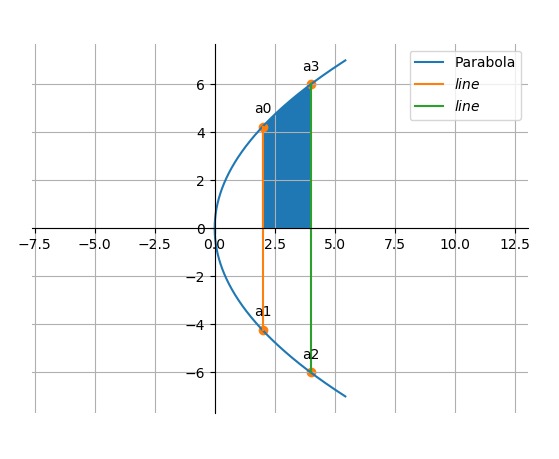
\includegraphics[width=0.75\columnwidth]{chapters/12/8/1/2/figs/conics1.png}
		\caption{}
		\label{fig:12/8/1/2}
  	\end{figure}
The parameters of the conic are
\begin{align}
 \vec{V} = \myvec{0 & 0\\0 & 1},
	\vec{u} = \frac{9}{2}\myvec{1 \\0},
 f = 0.
\end{align}
The parameters of 
the line $x-2=0$ are
\begin{align}
\vec{q_2}=\myvec{2\\0},
\vec{m_2}=\myvec{0\\1}
\end{align}
Substituting in 
\eqref{eq:tangent_roots},
\begin{align}
\kappa_i=\pm 3\sqrt{2}
\end{align}
yielding
\begin{align}
\vec{a_0}=\myvec{2\\3\sqrt{2}},
\vec{a_1}=\myvec{2\\-3\sqrt{2}}.
\end{align}
Similarly, 
for the line $x-4=0$,
\begin{align}
\vec{q_1}=\myvec{4\\0},
\vec{m_1}=\myvec{0\\1}
\end{align}
yielding
\begin{align}
\kappa_i=\pm 6.
\end{align}
Thus, 
\begin{align}
\vec{a_3}=\myvec{4\\6},
\vec{a_2}=\myvec{4\\-6}
\end{align}
and 
		from \figref{fig:12/8/1/2},
the 
desired area of the parabola is
\begin{align}
\int_{0}^{4} \ 3\sqrt{x} \,dx-\int_{0}^{2} \ 3\sqrt{x} \,dx
=16-4\sqrt{2}
\end{align}
